\begin{definition}
{\em Random Sampling :}
A collection of random variables $X_{1},X_{2},\dots,X_{n}$ is said to be a random sample of size $n$ if they are independent and identically distributed, i.e,
\begin{enumerate}
    \item $X_{1},X_{2},\dots,X_{n}$ are independent random variables
    \item They have the same distribution (Let us denote it by $F_{X}(x)$), i.e,
    \begin{align}
        F_{X}(x)=F_{X_{i}}(x), i = 1,2,\dots,n \forall x\in \mathbb{R}
    \end{align}
\end{enumerate}
\end{definition}
\begin{definition}
{\em Order Statistics :}
Given a random sample $X_{1},X_{2},\dots,X_{n}$, the sequence $X_{(1)},X_{(2)},\dots,X_{(n)}$ is called the order statistics of it. Here,
\begin{align}
    &X_{(1)}=\min\brak{X_{1},X_{2},\dots,X_{n}}\\
    &X_{(2)}=\text{the }2^{nd}\text{ smallest of }X_{1},X_{2},\dots,X_{n}\\
    &\vdots\\
    &X_{(n)}=\max\brak{X_{1},X_{2},\dots,X_{n}}
\end{align}
\end{definition}
\begin{lemma}
{\em Distribution of the maximum :}
\begin{align}
	\label{eq:conv/1/pdf}
    f_{T_{n}}(x)&=\begin{cases}
	nx^{n-1}, & 0< x<1 \\~\\[-1em]
	0, & otherwise
	\end{cases}\\
	F_{T_{n}}(x)&=\begin{cases}
	x^{n}, & 0< x<1 \\~\\[-1em]
	1, & x\geq 1\\~\\[-1em]
	0, & otherwise
	\end{cases} 
	\label{eq:conv/1/cdf}
\end{align}
\end{lemma}
%\proof
Proof:
\begin{align}
   F_{X_{(n)}}(x)&=\pr{X_{(n)}\leq x}\\
   &=\pr{X_{1}\leq x,X_{2}\leq x,\dots,X_{n}\leq x}\\
   &=\pr{X_{1}\leq x}\pr{X_{2}\leq x}\dots\pr{X_{n}\leq x}\\
   \label{conv/1/eq:F}
   &=\sbrak{\pr{X_{1}\leq x}}^{n}\brak{ \text{i.i.d}}\\
   &=\sbrak{F_{X}(x)}^{n}
   \label{eq:conv/1/cdf/max}
\end{align}
and 
\begin{align}
   f_{X_{(n)}}(x)&=\dfrac{d}{dx}\brak{F_{X_{(n)}}(x)}=\dfrac{d}{dx}\brak{\sbrak{F_{X}(x)}^{n}}\\
   &=n\brak{\sbrak{F_{X}(x)}^{n-1}}\dfrac{d}{dx}\brak{F_{X}(x)}\\
%   \label{conv/1/eq:f}
   &=n\sbrak{F_{X}(x)}^{n-1}f_{X}(x)
   \label{eq:conv/1/pdf/max}
\end{align}
$\because $
\begin{align}
    f_{X_{i}}(x)&=\begin{cases}
	1, & 0< x<1 \\~\\[-1em]
	0, & otherwise
	\end{cases},
	\\
	F_{X_{i}}(x)&=\begin{cases}
	x, & 0< x<1 \\~\\[-1em]
	1, & x\geq 1\\~\\[-1em]
	0, & otherwise,
	\end{cases} 
\end{align}
$\forall i\in \mathbb{N}$.  Substituting the above in    \eqref{eq:conv/1/pdf/max} and \eqref{eq:conv/1/cdf/max} yields 	\eqref{eq:conv/1/pdf} and 	\eqref{eq:conv/1/cdf} respectively. 
Then, as $T_{n}=max\{ X_{1},X_{2},\dots,X_{n}\}=X_{(n)}$,
\begin{lemma}
If $Y=aX+b$ and $a<0$, then
\begin{align}
\label{conv/1/eq:form}
    F_{Y}(y)=1-F_{X}\brak{\dfrac{y-b}{a}}
\end{align}
\end{lemma}
\begin{definition}
{\em	Convergence in Probability :}
A sequence of random variables $X_{1},X_{2},X_{3},\dots$ converges in probability to a random variable $X$, shown by $X_{n}\xrightarrow[]{p}X$, if
\begin{align}
    \displaystyle\lim_{n\to\infty}\pr{|X_{n}-X|\geq\epsilon}=0,\forall\epsilon>0
\end{align}
\end{definition}
%
\begin{definition}
	{\em Convergence in Distribution :}
A sequence of random variables $X_{1},X_{2},X_{3},\dots$ converges in distribution to a random variable $X$, shown by $X_{n}\xrightarrow[]{d}X$, if
\begin{align}
    \displaystyle\lim_{n\to\infty}F_{X_{n}}(x)=F_{X}(x)
\end{align}
for all $x$ at which $F_{X}(x)$ is continuous.
\end{definition}
%
\begin{enumerate}
\item 
%To evaluate : $\displaystyle\lim_{n\to\infty}\pr{|T_{n}-1|\geq\epsilon},\forall\epsilon>0$
\begin{multline}
    \displaystyle\lim_{n\to\infty}\pr{|T_{n}-1|\geq\epsilon}=\displaystyle\lim_{n\to\infty}\pr{1-T_{n}\geq\epsilon}\\
	=\displaystyle\lim_{n\to\infty}\pr{T_{n}\leq1-\epsilon}=\displaystyle\lim_{n\to\infty}F_{T_{n}}(1-\epsilon)
	\label{conv/1/1/cdf}
\end{multline}
\begin{align}
    \because F_{T_{n}}(1-\epsilon)=\begin{cases}
	(1-\epsilon)^{n}, & 0< \epsilon<1 \\~\\[-1em]
	0, & \epsilon\geq 1
	\end{cases}
	\label{conv/1/1/cdf/epsilon}
\end{align}
and 
\begin{align}
	\label{conv/1/1/cdf/epsilon/lim}
    \because\displaystyle\lim_{n\to\infty}(1-\epsilon)^{n}=0 \text{ for } 0< \epsilon<1\\
\end{align}
%
from 	\eqref{conv/1/1/cdf/epsilon/lim}, 	\eqref{conv/1/1/cdf/epsilon} and 	\eqref{conv/1/1/cdf},
\begin{align}
	 \displaystyle\lim_{n\to\infty}\pr{|T_{n}-1|\geq\epsilon}=0,\forall\epsilon>0
\end{align}
$\therefore T_{n}$ converges to 1 in probability.
\item 
Substituting $a=-n,b=n$ in \eqref{conv/1/eq:form},
\begin{align}
	F_{n(1-T_{n})}(x)=1-F_{T_{n}}\brak{1-\dfrac{x}{n}}\\
\end{align}	
where
\begin{align}
    F_{T_{n}}\brak{1-\dfrac{x}{n}}=\begin{cases}
	\brak{1-\dfrac{x}{n}}^{n}, & 0< x<n \\~\\[-1em]
	1, & x\leq 0\\~\\[-1em]
	0, & x\geq n
	\end{cases} \\
	from  	\eqref{eq:conv/1/cdf}
\end{align}
\begin{align}
	\because\displaystyle\lim_{n\to\infty}\brak{1-\dfrac{y}{n}}^{n}=e^{-y}, \\
\end{align}
\begin{align}
\therefore\displaystyle\lim_{n\to\infty} F_{T_{n}}\brak{1-\dfrac{x}{n}}&=\begin{cases}
	e^{-x}, & x>0 \\~\\[-1em]
	1, & x\leq 0
	\end{cases} \\
	\implies 
	\displaystyle\lim_{n\to\infty}F_{n(1-T_{n})}(x)&=1-\displaystyle\lim_{n\to\infty} F_{T_{n}}\brak{1-\dfrac{x}{n}}
\end{align}
which can be expressed as
\begin{align}
\label{conv/1/eq:cdf1}
    \therefore\displaystyle\lim_{n\to\infty} F_{n(1-T_{n})}(x)=\begin{cases}
	1-e^{-x}, & x>0 \\~\\[-1em]
	0, & x\leq 0
	\end{cases} 
\end{align}
$\therefore n(1-T_{n})$ converges in distribution to the random variable $X\sim Exponential(1)$.
% \begin{figure}[h!]
% \centering
% 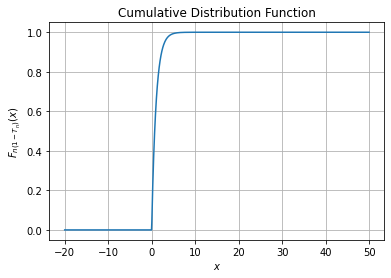
\includegraphics[width=\linewidth]{Assignment9}
% \caption{CDF}
% \label{conv/1/plot}
% \end{figure}
\item 
Substituting $a=-n^{2},b=n^{2}$ in \eqref{conv/1/eq:form},
\begin{align}
    F_{n^{2}(1-T_{n})}(x)&=1-F_{T_{n}}\brak{1-\dfrac{x}{n^{2}}}\\
    F_{T_{n}}\brak{1-\dfrac{x}{n^{2}}}&=\begin{cases}
	\brak{1-\dfrac{x}{n^{2}}}^{n}, & 0< x<n^{2} \\~\\[-1em]
	1, & x\leq 0\\~\\[-1em]
	0, & x\geq n^{2}
	\end{cases} \\
	&=\begin{cases}
		1, & x>0 \\~\\[-1em]
		1, & x\leq 0
		\end{cases} 
	\end{align}
	\begin{align}
	\because\displaystyle\lim_{n\to\infty}\brak{1-\dfrac{x}{n^{2}}}^{n}=1
%&\therefore\displaystyle\lim_{n\to\infty} F_{T_{n}}\brak{1-\dfrac{x}{n^{2}}}
	\end{align}
	yielding 
	\begin{align}
%&\because\displaystyle\lim_{n\to\infty}F_{n^{2}(1-T_{n})}(x)=1-\displaystyle\lim_{n\to\infty} F_{T_{n}}\brak{1-\dfrac{x}{n^{2}}}\\
\label{conv/1/eq:cdf2}
    \displaystyle\lim_{n\to\infty} F_{n^{2}(1-T_{n})}(x)=\begin{cases}
	0, & x>0 \\~\\[-1em]
	0, & x\leq 0
	\end{cases} 
\end{align}
which is not a valid CDF.  Hence, 
%$\because$ The CDF in \eqref{conv/1/eq:cdf2} is not valid,\\
$ n^{2}(1-T_{n})$ does not converge in distribution.
\item 
% Convergence in Probability :\\
% A sequence of random variables $X_{1},X_{2},X_{3},\dots$ converges in probability to a random variable $X$, shown by $X_{n}\xrightarrow[]{p}X$, if
% \begin{align}
%     \displaystyle\lim_{n\to\infty}\pr{|X_{n}-X|\geq\epsilon}=0,\forall\epsilon>0
% \end{align}
% To evaluate :\\ $\displaystyle\lim_{n\to\infty}\pr{|\sqrt{n}(1-T_{n})-0|\geq\epsilon},\forall\epsilon>0$
\begin{multline}
	\displaystyle\lim_{n\to\infty}\pr{|\sqrt{n}(1-T_{n})-0|\geq\epsilon}    \\ =\displaystyle\lim_{n\to\infty}\pr{1-T_{n}\geq\dfrac{\epsilon}{\sqrt{n}}}\\
    =\displaystyle\lim_{n\to\infty}\pr{T_{n}\leq1-\dfrac{\epsilon}{\sqrt{n}}}\\
	=\displaystyle\lim_{n\to\infty}F_{T_{n}}\brak{ 1-\dfrac{\epsilon}{\sqrt{n}}}
	\\
	=\begin{cases}
		\brak{1-\dfrac{\epsilon}{\sqrt{n}}}^{n}, & 0< \epsilon< \sqrt{n}\\~\\[-1em]
		0, & \epsilon\geq \sqrt{n}
		\end{cases}
\end{multline}
\begin{multline}
%    &F_{T_{n}}\brak{1-\dfrac{\epsilon}{\sqrt{n}}}\\
    \because\displaystyle\lim_{n\to\infty}\brak{1-\dfrac{\epsilon}{\sqrt{n}}}^{n}=0 \text{ for } 0< \epsilon<\sqrt{n},\\
     \displaystyle\lim_{n\to\infty}\pr{|\sqrt{n}(1-T_{n})-0|\geq\epsilon}=0,\forall\epsilon>0
\end{multline}
$\therefore\sqrt{n}(1-T_{n})$ converges to 0 in probability.
\end{enumerate}
\begin{lstlisting}
Hence, options 1), 2), 4) are correct.
\end{lstlisting}